%  pk-EFM theory paper
%  Created by Ryan P. Dwyer July 8, 2016

% %%   PREAMBLE   %%%

% PREPRINT
%\RequirePackage[displaymath,mathlines]{lineno}  % implement numbered lines
%\documentclass[aps,prl,preprint,citeautoscript,superscriptaddress,byrevtex,nofootinbib]{revtex4}
\documentclass[xcolor={dvipsnames}]{beamer}
\usepackage{presentation}
\usetheme{Boadilla}
\usecolortheme{beaver}
\setbeamertemplate{itemize items}[circle]

% GALLEY
%\RequirePackage[displaymath,mathlines]{lineno}  % implement numbered lines -- pagewise for two-column mode
% \documentclass[10pt,aps,prl,twocolumn,galley,citeautoscript,superscriptaddress,byrevtex,nofootinbib,nobalancelastpage,floatfix]{revtex4}

% TWO COLUMN
%\RequirePackage[displaymath,mathlines,pagewise]{lineno}  % implement numbered lines -- pagewise for two-column mode
%\RequirePackage[displaymath,mathlines]{lineno}  % implement numbered lines -- pagewise for two-column mode
% \documentclass[aps,prl,twocolumn,citeautoscript,superscriptaddress,byrevtex,nofootinbib,nobalancelastpage,floatfix]{revtex4}

% PACKAGES

\usepackage{siunitx}    % package for \meter etc
\usepackage{graphicx}         % \includegraphics{}
\usepackage{array}
\usepackage{mathtools}
\usepackage{amsmath,amsfonts,amssymb,amsthm} % For math equations, theorems, sy
\makeatletter
\def\zz\ignorespaces{\@ifnextchar-{}{\phantom{-}}}
\newcolumntype{C}{>{\zz}{c}}
\makeatother
\usepackage{bm}                       % need for bold greek letters
\usepackage{mciteplus}
\usepackage{caption}
\usepackage{booktabs}
\captionsetup{font=scriptsize,labelfont=scriptsize}
\usepackage{natbib}  % bibliography
%\RequirePackage{lineno}
       


% FONTS

% Computer Modern is the default LaTeX font.
% Uncomment one of the lines below to try another font.
% PRL actually appears to use a font closet to Times.
% \usepackage{times}     % ~not~ computer modern fonts
\usepackage{palatino}  % ~not~ computer modern fonts

% FORMATTING OPTIONS

\lefthyphenmin=3           % Fix LaTeX hyphenation
\righthyphenmin=4          % Fix LaTeX hyphenation
%\setlength{\parskip}{6pt}  % Set paragraph spacing to be easy on the eyes

\graphicspath{
{/Users/ryandwyer/Dropbox/_JAM_MS__Dwyer201607__pk_EFM_theory__figs/}
}

% COMMANDS
\newcommand{\trimcaptionspacing}{\vspace{-0.25in}}      % include in figures to decrease the text-to-figure spacing
\newcommand{\trimcaptionspacinghalf}{\vspace{-0.10in}}  % include in figures to decrease the text-to-figure spacing
\def\bibfont{\footnotesize} % Smaller font in the bibliography

% Easy text subscripts
\newcommand{\st}[1]{_\text{#1}}


% See http://tex.stackexchange.com/questions/21598/how-to-color-math-symbols
\makeatletter
\def\mathcolor#1#{\@mathcolor{#1}}
\def\@mathcolor#1#2#3{%
  \protect\leavevmode
  \begingroup
    \color#1{#2}#3%
  \endgroup
}
\makeatother

 
 
 
%Information to be included in the title page:

\title[What is the SVD?]{What is the singular value decomposition?}

\author{Ryan Dwyer \inst{1}}

\institute[]{
    \inst{1} Department of Chemistry and Chemical Biology \\
    Cornell University}

\date[2016.11.07]{Marohn Group Meeting \\
November 7, 2016}

\begin{document}

\frame{\titlepage}

\begin{frame}
\frametitle{Applications of the singular value decomposition}
\begin{itemize}
    \item Linear least squares solution (pseudoinverse)
    \item Approximating matrices
    \item Optimization
    \item Recommender systems (Netflix, PageRank)
    \item Quantum information (Schmidt decomposition)
\end{itemize}
\end{frame}


% \item 
% 
% 
% \end{equation}

\begin{frame}
\frametitle{Matrix decompositions make certain operations easy}
\begin{exampleblock}{Analogy: Eigendecomposition}
\begin{align*}
\underbrace{A^n = A A \ldots = \; ? \tfrac{}{}}_\text{$n$ matrix multiplications: slow, obtuse}& & \underbrace{e^{A t} = I + A t + \tfrac{1}{2} A^2 t^2 + \ldots = \; ?}_\text{power series: potentially even worse!}
\end{align*}
\begin{align*}
A& = Q \Lambda Q^{-1} \Rightarrow & & \underbrace{A^n = Q \Lambda^n Q^{-1}, \quad e^{At} = Q e^{\Lambda} Q^{-1}}_\text{scalar functions: fast, understandable}
\end{align*}
\begin{itemize}
    \item Eigendecomposition diagonalizes square $n \times n$ matrices
    \item Matrix multiplication or power series $\Rightarrow$ scalar function evaluation
    \item Solution of differential and difference equations, Markov chains
\end{itemize}
\end{exampleblock}
\end{frame}

% \begin{frame}
% SVD compactly describes how a matrix $A$ transforms vectors $\mathbf{x}$ to vectors $\mathbf{y}$,
% \begin{equation}
% \mathbf{y} = A \mathbf{x}
% \end{equation}
% \end{frame}

\begin{frame}
\frametitle{Singular value decomposition}
Understand how $m \times n$ matrices $A$ transform $n$-dimensional $\mathbf{x}$ to $m$-dimensional $\mathbf{y}$.
\begin{equation*}
\mathbf{y} = A \mathbf{x}
\end{equation*}
\begin{itemize}
    \item How does a small change $\delta \mathbf{x}$ affect $\mathbf{y}$?
    \item How does a small change $\delta \mathbf{y}$ affect $\mathbf{x}$?
    \item Is $A$ singular or \emph{almost} singular?
    \item How well can $A$ be approximated / compressed?
\end{itemize}
\end{frame}

\begin{frame}
\frametitle{Problems that can be formulated $\mathbf{y} = A \mathbf{x}$}
\begin{exampleblock}{Examples}
\begin{table}[h!]
\centering
\resizebox{\columnwidth}{!}{ %
\begin{tabular}{ccccc}

Problem & $\mathbf{y}$ & $A$ & $\mathbf{x}$ \\ \midrule
\begin{minipage}[t]{1.75in}%
Ordinary least squares (e.g., line fit)%
\end{minipage} & 
Data, $\begin{pmatrix} y(t_1) \\ y(t_2) \\ \vdots \end{pmatrix}$& 
$\begin{pmatrix}1 & t_1 \\ 1 & t_2 \\ \vdots & \vdots \end{pmatrix}$ & $\begin{pmatrix} b \\ m \end{pmatrix}$, fit parameters &  \\
\begin{minipage}[t]{1.75in}%
Non-linear least squares (e.g., exponential fit)%
\end{minipage}&
Residuals, $\begin{pmatrix} y(t_1) - f(t_1, \mathbf{x}_0) \\ y(t_2) - f(t_2, \mathbf{x}_0) \\ \vdots \end{pmatrix}$& 
$\nabla f(\mathbf{x}_0)$ &
$\begin{pmatrix} \delta y_0 \\ \delta \tau \end{pmatrix}$, change in fit param.
\\
\begin{minipage}[t]{1.75in}%
Convolution,
$y = H \ast x$%
\end{minipage}
 & Output, $\begin{pmatrix} y(t_{k}) \\ y(t_{k+1}) \\ \vdots \end{pmatrix}$&%
\begin{minipage}{0.6in}%
\centering%
Toeplitz matrix for $H$%
\end{minipage} & Input, $\begin{pmatrix} x(t_1) \\ x(t_2) \\ \vdots \end{pmatrix}$
\end{tabular}
%
}
\end{table}
\end{exampleblock}
\pause
\begin{block}{}
\centering
Majority of scientists' data analysis and signal processing

falls into one of these categories!
\end{block}
\end{frame}


\begin{frame}
\frametitle{Singular value decomposition}
\begin{itemize}
    \item SVD decomposes an $m \times n$ matrix A into,
\begin{equation}
A = U \Sigma V^T
\end{equation}
    \item $V$, $U$ orthonormal bases for $\mathbf{x}$, $\mathbf{y}$
    \item $\Sigma$ a diagonal matrix of \emph{positive} singular values
\end{itemize}
\begin{figure}
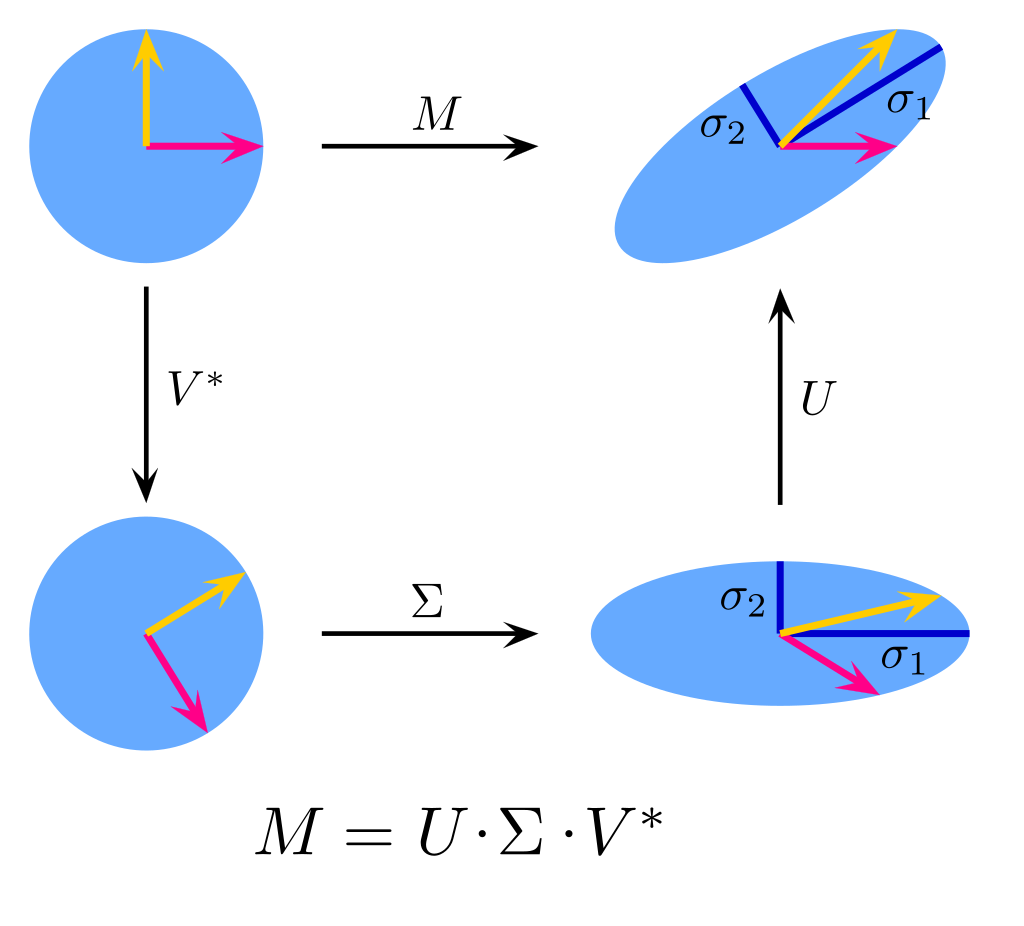
\includegraphics[width=2in]{figs/Singular-Value-Decomposition.png}
\caption{By Georg-Johann - Own work, CC BY-SA 3.0, https://commons.wikimedia.org/w/index.php?curid=11342212}
\end{figure}
\end{frame}


% \begin{frame}
% \frametitle{Action of a matrix}
% \begin{figure}
% 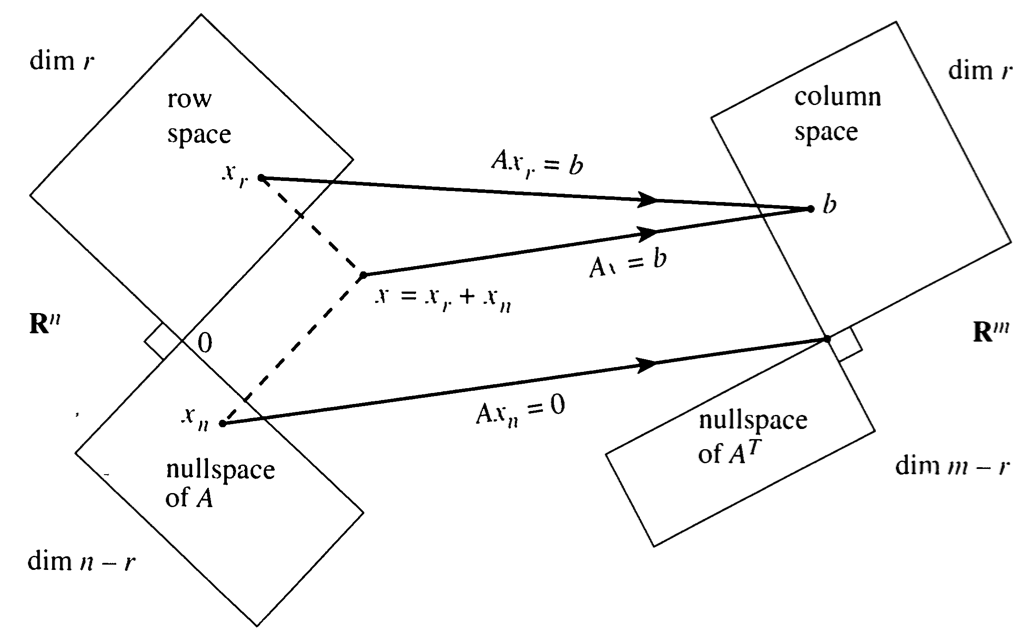
\includegraphics[width=3.75in]{figs/Strang1993nov-fig1.png}
% \end{figure}
% \end{frame}


\begin{frame}
\frametitle{Example: Exponential decay curve fitting}
\begin{columns}
    \column{0.3\textwidth}
        \begin{block}{}
        How does changing parameters affect the best-fit result?
        \end{block}
        \begin{block}{}
        How does changing data affect the parameter values?
        \end{block}

    \column{0.68\textwidth}
    \begin{figure}
        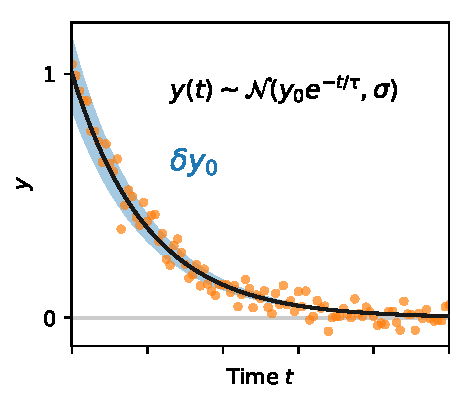
\includegraphics[width=\textwidth]{figs/dA.pdf}
    \end{figure}

\end{columns}
\end{frame}

\begin{frame}
\frametitle{Example: Exponential decay curve fitting}
\begin{columns}
    \column{0.3\textwidth}
        \begin{block}{}
        How does changing parameters affect the best-fit result?
        \end{block}
        \begin{block}{}
        How does changing data affect the parameter values?
        \end{block}

    \column{0.68\textwidth}
    \begin{figure}
        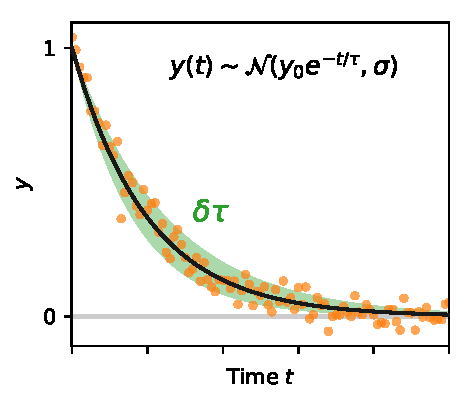
\includegraphics[width=\textwidth]{figs/dtau.pdf}
    \end{figure}

\end{columns}
\end{frame}

\begin{frame}
\frametitle{Linearize the equation about a point}
\begin{columns}
    \column{0.25\textwidth}
        \begin{align*}
        \mathbf{y}& = f(\mathbf{x}) \\
        \delta \mathbf{y}& \approx \nabla f(\mathbf{x}_0) \delta \mathbf{x} \\
        J& = \nabla f(\mathbf{x}_0) \\
        \mathbf{x}& = (y_0 \; \; \tau)^T
        \end{align*}

    \column{0.75\textwidth}
        \begin{figure}
        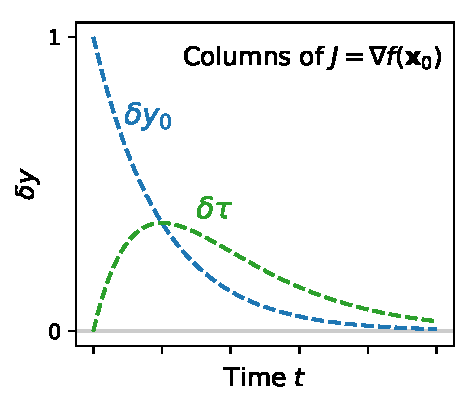
\includegraphics[width=\textwidth]{figs/dy0dtau.pdf}
        \end{figure}
\end{columns}
\end{frame}

\begin{frame}
\frametitle{How does $y$ affect the parameters?}
\begin{figure}
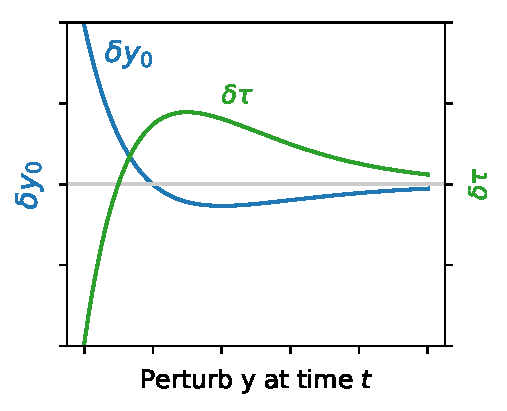
\includegraphics[width=0.95\textheight]{figs/perturb-y.pdf}
\end{figure}
\end{frame}

\begin{frame}
\frametitle{Compare:}
\begin{columns}
    \column{0.45\textwidth}
    \begin{figure}
        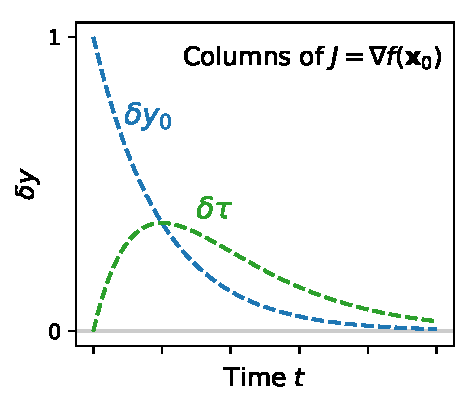
\includegraphics[width=\textwidth]{figs/dy0dtau.pdf}
    \end{figure}
    \column{0.45\textwidth}
    \begin{figure}
        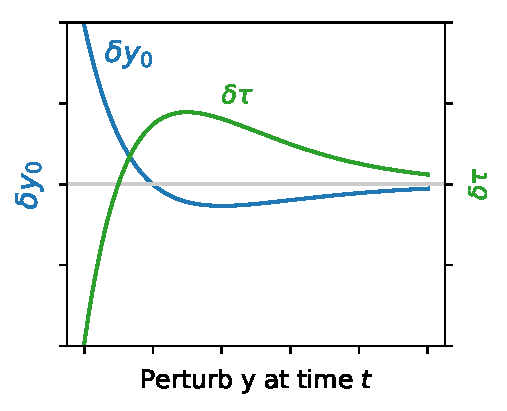
\includegraphics[width=\textwidth]{figs/perturb-y.pdf}
    \end{figure}
\end{columns}
These relationships are complicated and hard to describe because $(y_0 \; \; \tau)^T$
and $\left( f(t_0) \; \; f(t_1) \; \; f(t_2) \right)^T$ are poor bases to describe the \emph{action} of the matrix $J$.
\end{frame}

\begin{frame}
\frametitle{Singular value decomposition}
\begin{figure}
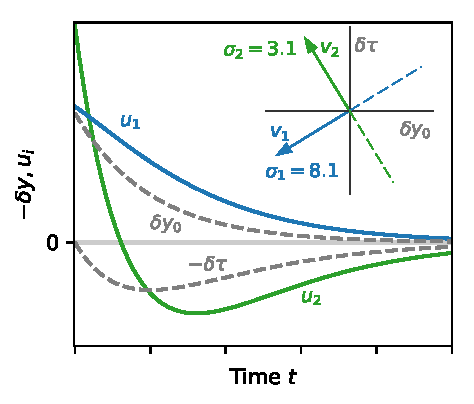
\includegraphics[height=0.9\textheight]{figs/dy-usv.pdf}
\end{figure}
\end{frame}

\begin{frame}
\frametitle{Extension: double exponential curve fit}
\begin{block}{Problem}
Double exponential fitting is ``ill-conditioned.'' Why?
\end{block}
\begin{figure}
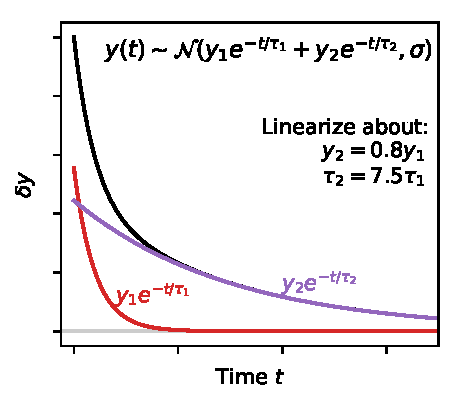
\includegraphics[height=0.7\textheight]{figs/two-time-constants.pdf}
\end{figure}
\end{frame}

\begin{frame}
\frametitle{Extension: double exponential curve fit}
\begin{columns}
    \column{0.25\textwidth}
    \begin{align*}
    \mathbf{y}& = f(\mathbf{x}) \\
    \delta \mathbf{y}& \approx \nabla f(\mathbf{x}_0) \delta \mathbf{x} \\
    J& = \nabla f(\mathbf{x}_0) \\
    \mathbf{x}& = \begin{pmatrix}
    y_1 \\
    y_2 \\
    \tau_1 \\
    \tau_2
    \end{pmatrix}
    \end{align*}

    \column{0.75\textwidth}
    \begin{figure}
    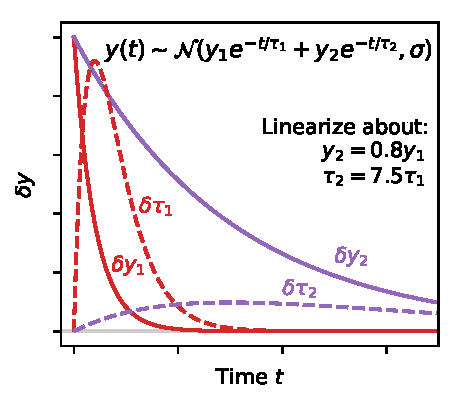
\includegraphics[width=\textwidth]{figs/two-time-constants-Jac.pdf}
    \end{figure}
\end{columns}
\end{frame}


\begin{frame}
\frametitle{SVD of double exponential}
\vspace{-0.25in}
\begin{columns}
    \column{0.58\textwidth}
    \begin{figure}
    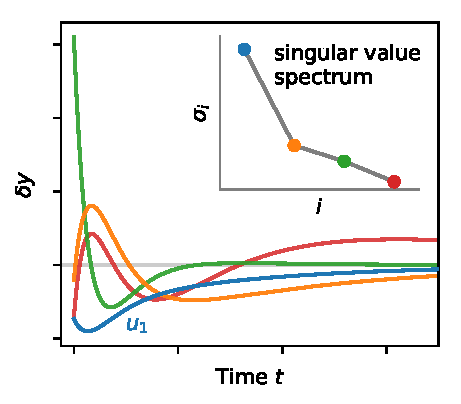
\includegraphics[width=\textwidth]{figs/double-expon-svd.pdf}
    \end{figure}
    \vspace{-0.3in}
    \begin{block}{}
    99.7\% energy in first 3 singular values.

    Jacobian $J$ is ``almost'' singular.

    Data $y$ gives almost no information on second time constant $\tau_2$.
    \end{block}

    \column{0.4\textwidth}
    \vspace{-0.35in}
    \begin{figure}
    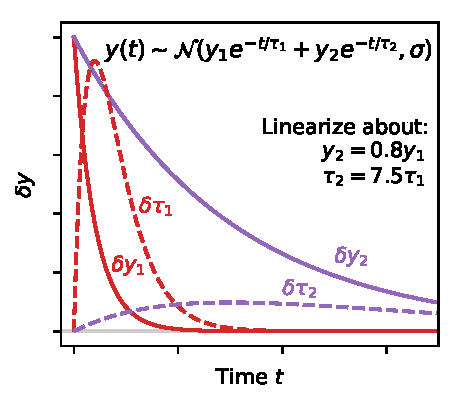
\includegraphics[width=1.07\textwidth]{figs/two-time-constants-Jac.pdf}
    \end{figure}
    \begin{equation*}
    \begin{matrix*}[C]
    & v_1 & v_2 & v_3 & v_4 \\
\delta y_1& -2& 4& 9& 2 \\
\delta y_2& -8& -5& 0& -3 \\
\delta \tau_1& -5& 7& -5& 2 \\
\delta \tau_2& -1& -4& -1& \mathcolor{purple}{9} \\
    \end{matrix*}
    \end{equation*}



\end{columns}
\end{frame}

\begin{frame}
\frametitle{Optimization applications: least squares}
\begin{itemize}
    \item Consider data $y$ fit to $A x$, where $x$ is a vector of parameters
    \item Define vector of residuals $r$,
    $$r = y - A x$$
    \item Objective: minimize square of residuals
\begin{align*}
\min_{x} f(x)& = \frac{1}{2} \lVert r \rVert^2 = \frac{1}{2} r^T r 
\end{align*}
\end{itemize}
\begin{block}{What is special about least squares problems?}
Residuals give ``free'' information about derivatives
\end{block}
\end{frame}

\begin{frame}
\frametitle{Optimization applications: least squares}
\begin{exampleblock}{Gradient}
By the chain rule,
\begin{align*}
 \nabla f = - A^T r,
\end{align*}
Residuals projected back to the space of $x$ with $A^T$ is the steepest descent direction.
\end{exampleblock}
\begin{exampleblock}{Hessian}
$$\nabla^2 f = A^T A $$

In non-linear least squares, Jacobian of residuals $J$ gives a good guess for the Hessian.
\end{exampleblock}
\end{frame}

\begin{frame}
\frametitle{Optimization applications: least squares}
\begin{figure}
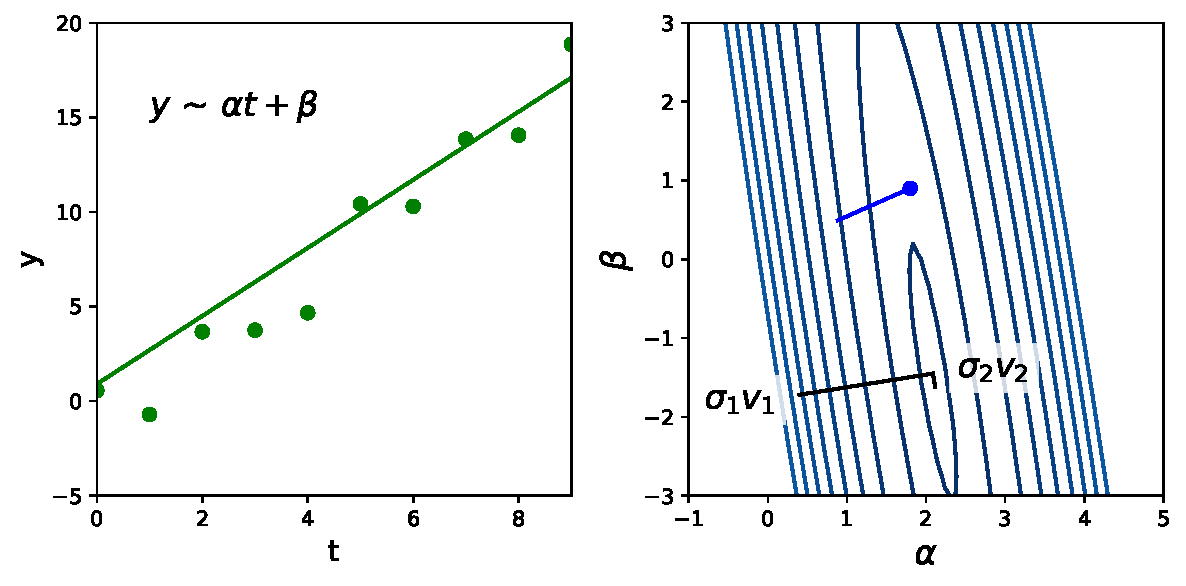
\includegraphics[width=\textwidth]{figs/linear_fit.pdf}
\end{figure}
\begin{equation*}
\frac{1}{2} r^T r = \frac{1}{2} x^T A^T A x + y^T A x + y^T y
\end{equation*}
\end{frame}

\begin{frame}
\frametitle{Optimization applications: Landweber iteration}
Choose the next value of the parameter vector $x$ using,
\begin{align*}
x_{k+1}& = x_k + \alpha \, A^T r_k 
\end{align*}
\begin{block}{}
This is gradient descent with a fixed step size, using the residuals $r$ to compute the gradient direction (since $\nabla f(x_k) = - A^T r_k$)
\end{block}
\end{frame}

\begin{frame}
\frametitle{Stability of Landweber iteration}
\begin{columns}
\column{0.46\textwidth}
Define the error vector $e_k$,
$$e_k = x^+ - x_k$$
\begin{itemize}
    \item $x^+$: least squares solution 
    \item $x_k$:  $k^\text{th}$ parameter vector
\end{itemize}
The Landweber iteration can be written as,
\begin{align*}
x_{k+1}& = x^+ - e_{k+1} = x^+ - e_k + \alpha \, A^T A e_k \\
e_{k+1}& = (I - \alpha A^T A) e_k
\end{align*}
\column{0.46\textwidth}
For an initial guess of $\mathbf{0}$, the initial error is $x^+$, so
$$ x_{k} = (I - (\alpha A^T A)^k) x^+ $$
This corresponds to pulling in components of the SVD,
$$  x_{k} = V (I - (\alpha \Sigma^2)^k) V^T x^+  $$
\end{columns}
\end{frame}



% \end{frame}

% \begin{frame}
% \frametitle{Examples}
% \begin{figure}
% 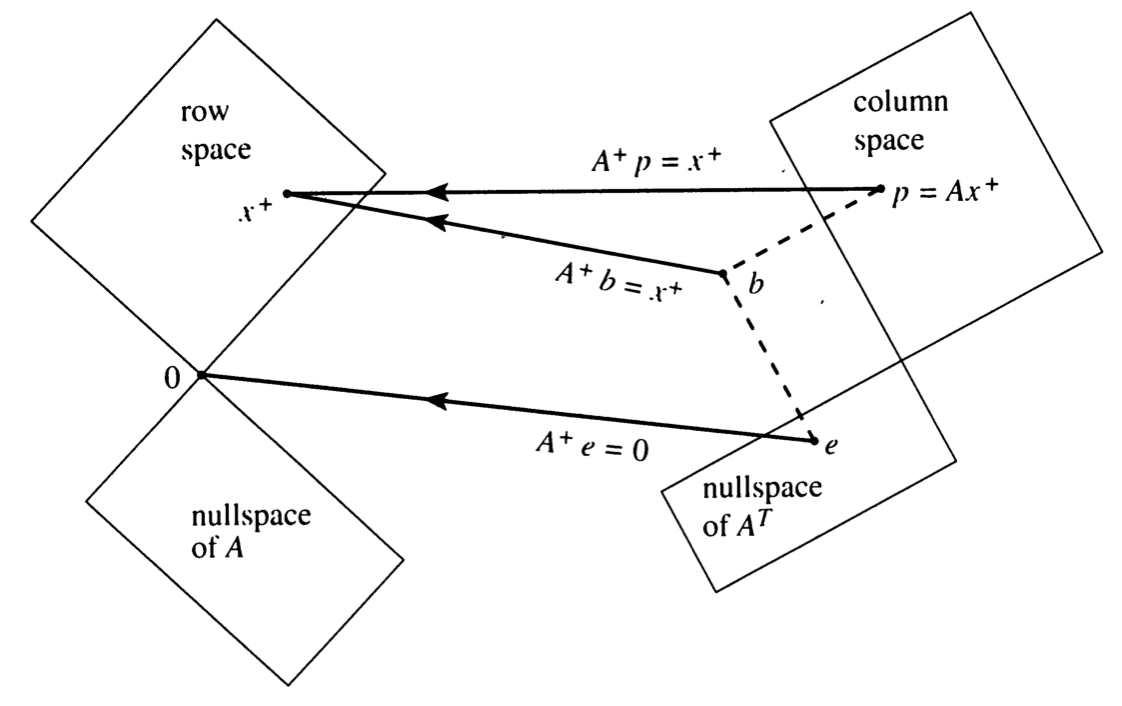
\includegraphics[width=3in]{figs/Strang1993nov-fig4.png}
% \end{figure}
% Linear least squares:
% \begin{equation}
% y = \begin{pmatrix}
% -1 & 1 \\
% 0 & 1 \\
% 1 & 1 \\
% \end{pmatrix}
% \begin{pmatrix}
% \alpha \\
% \beta
% \end{pmatrix}
% \end{equation}
% \end{frame}

% \begin{frame}
% \frametitle{Examples}
% \begin{figure}
% 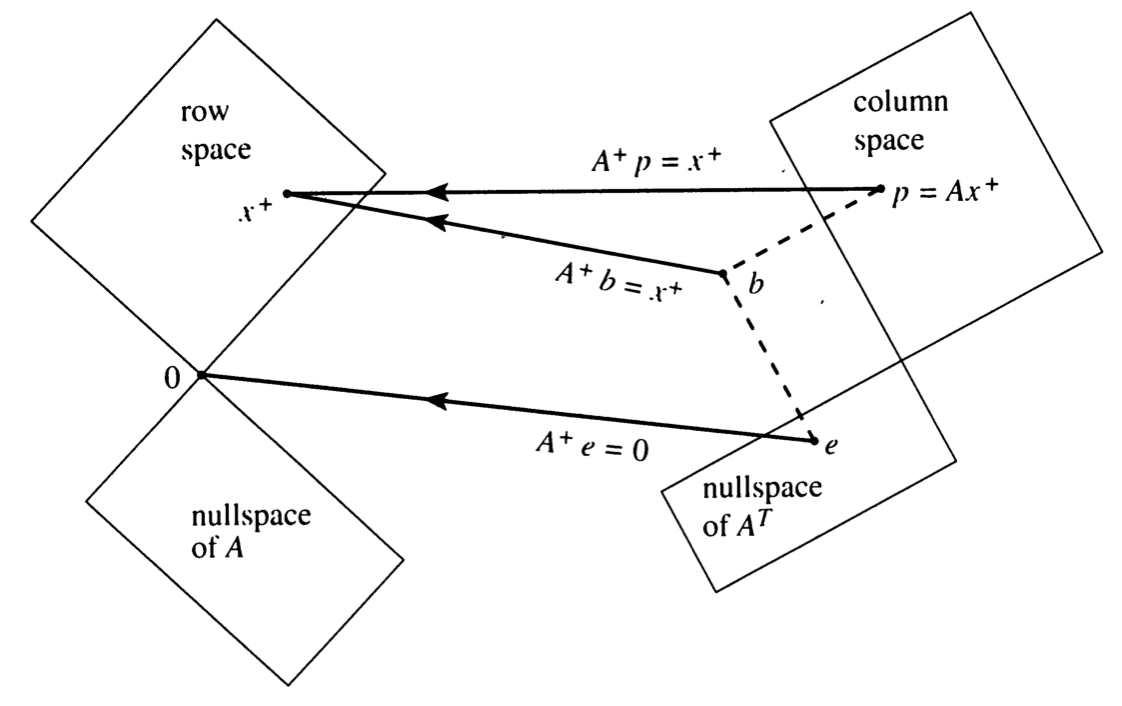
\includegraphics[width=3in]{figs/Strang1993nov-fig4.png}
% \end{figure}
% Linear least squares:
% \begin{equation}
% A = \begin{pmatrix}
% -1/\sqrt{3} & -1/\sqrt{2} \\
% -1/\sqrt{3} & 0 \\
% -1/\sqrt{3} & 1/\sqrt{2}
% \end{pmatrix}
% \begin{pmatrix}
%     \sqrt{3}
% \end{pmatrix}
% \begin{pmatrix}
% \alpha \\
% \beta
% \end{pmatrix}
% \end{equation}
% \end{frame}



% =========================
% \def\bibsection{\vspace{6pt}}
% \setlength{\bibsep}{0pt}

% \bibliographystyle{bst/naturemag_jm}

% \bibliography{bib/jam99_2012-03-29_Ryan}
% \label{TheEnd}
\end{document}
